\documentclass[1p]{elsarticle_modified}
%\bibliographystyle{elsarticle-num}

%\usepackage[colorlinks]{hyperref}
%\usepackage{abbrmath_seonhwa} %\Abb, \Ascr, \Acal ,\Abf, \Afrak
\usepackage{amsfonts}
\usepackage{amssymb}
\usepackage{amsmath}
\usepackage{amsthm}
\usepackage{scalefnt}
\usepackage{amsbsy}
\usepackage{kotex}
\usepackage{caption}
\usepackage{subfig}
\usepackage{color}
\usepackage{graphicx}
\usepackage{xcolor} %% white, black, red, green, blue, cyan, magenta, yellow
\usepackage{float}
\usepackage{setspace}
\usepackage{hyperref}

\usepackage{tikz}
\usetikzlibrary{arrows}

\usepackage{multirow}
\usepackage{array} % fixed length table
\usepackage{hhline}

%%%%%%%%%%%%%%%%%%%%%
\makeatletter
\renewcommand*\env@matrix[1][\arraystretch]{%
	\edef\arraystretch{#1}%
	\hskip -\arraycolsep
	\let\@ifnextchar\new@ifnextchar
	\array{*\c@MaxMatrixCols c}}
\makeatother %https://tex.stackexchange.com/questions/14071/how-can-i-increase-the-line-spacing-in-a-matrix
%%%%%%%%%%%%%%%

\usepackage[normalem]{ulem}

\newcommand{\msout}[1]{\ifmmode\text{\sout{\ensuremath{#1}}}\else\sout{#1}\fi}
%SOURCE: \msout is \stkout macro in https://tex.stackexchange.com/questions/20609/strikeout-in-math-mode

\newcommand{\cancel}[1]{
	\ifmmode
	{\color{red}\msout{#1}}
	\else
	{\color{red}\sout{#1}}
	\fi
}

\newcommand{\add}[1]{
	{\color{blue}\uwave{#1}}
}

\newcommand{\replace}[2]{
	\ifmmode
	{\color{red}\msout{#1}}{\color{blue}\uwave{#2}}
	\else
	{\color{red}\sout{#1}}{\color{blue}\uwave{#2}}
	\fi
}

\newcommand{\Sol}{\mathcal{S}} %segment
\newcommand{\D}{D} %diagram
\newcommand{\A}{\mathcal{A}} %arc


%%%%%%%%%%%%%%%%%%%%%%%%%%%%%5 test

\def\sl{\operatorname{\textup{SL}}(2,\Cbb)}
\def\psl{\operatorname{\textup{PSL}}(2,\Cbb)}
\def\quan{\mkern 1mu \triangleright \mkern 1mu}

\theoremstyle{definition}
\newtheorem{thm}{Theorem}[section]
\newtheorem{prop}[thm]{Proposition}
\newtheorem{lem}[thm]{Lemma}
\newtheorem{ques}[thm]{Question}
\newtheorem{cor}[thm]{Corollary}
\newtheorem{defn}[thm]{Definition}
\newtheorem{exam}[thm]{Example}
\newtheorem{rmk}[thm]{Remark}
\newtheorem{alg}[thm]{Algorithm}

\newcommand{\I}{\sqrt{-1}}
\begin{document}

%\begin{frontmatter}
%
%\title{Boundary parabolic representations of knots up to 8 crossings}
%
%%% Group authors per affiliation:
%\author{Yunhi Cho} 
%\address{Department of Mathematics, University of Seoul, Seoul, Korea}
%\ead{yhcho@uos.ac.kr}
%
%
%\author{Seonhwa Kim} %\fnref{s_kim}}
%\address{Center for Geometry and Physics, Institute for Basic Science, Pohang, 37673, Korea}
%\ead{ryeona17@ibs.re.kr}
%
%\author{Hyuk Kim}
%\address{Department of Mathematical Sciences, Seoul National University, Seoul 08826, Korea}
%\ead{hyukkim@snu.ac.kr}
%
%\author{Seokbeom Yoon}
%\address{Department of Mathematical Sciences, Seoul National University, Seoul, 08826,  Korea}
%\ead{sbyoon15@snu.ac.kr}
%
%\begin{abstract}
%We find all boundary parabolic representation of knots up to 8 crossings.
%
%\end{abstract}
%\begin{keyword}
%    \MSC[2010] 57M25 
%\end{keyword}
%
%\end{frontmatter}

%\linenumbers
%\tableofcontents
%
\newcommand\colored[1]{\textcolor{white}{\rule[-0.35ex]{0.8em}{1.4ex}}\kern-0.8em\color{red} #1}%
%\newcommand\colored[1]{\textcolor{white}{ #1}\kern-2.17ex	\textcolor{white}{ #1}\kern-1.81ex	\textcolor{white}{ #1}\kern-2.15ex\color{red}#1	}

{\Large $\underline{12a_{0974}~(K12a_{0974})}$}

\setlength{\tabcolsep}{10pt}
\renewcommand{\arraystretch}{1.6}
\vspace{1cm}\begin{tabular}{m{100pt}>{\centering\arraybackslash}m{274pt}}
\multirow{5}{120pt}{
	\centering
	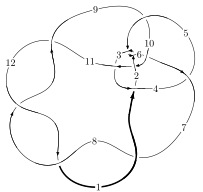
\includegraphics[width=112pt]{../../../GIT/diagram.site/Diagrams/png/1775_12a_0974.png}\\
\ \ \ A knot diagram\footnotemark}&
\allowdisplaybreaks
\textbf{Linearized knot diagam} \\
\cline{2-2}
 &
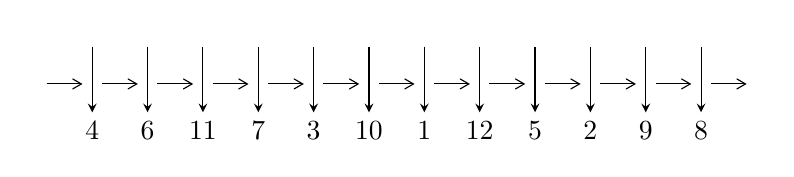
\begin{tikzpicture}[x=20pt, y=17pt]
	% nodes
	\node (C0) at (0, 0) {};
	\node (C1) at (1, 0) {};
	\node (C1U) at (1, +1) {};
	\node (C1D) at (1, -1) {4};

	\node (C2) at (2, 0) {};
	\node (C2U) at (2, +1) {};
	\node (C2D) at (2, -1) {6};

	\node (C3) at (3, 0) {};
	\node (C3U) at (3, +1) {};
	\node (C3D) at (3, -1) {11};

	\node (C4) at (4, 0) {};
	\node (C4U) at (4, +1) {};
	\node (C4D) at (4, -1) {7};

	\node (C5) at (5, 0) {};
	\node (C5U) at (5, +1) {};
	\node (C5D) at (5, -1) {3};

	\node (C6) at (6, 0) {};
	\node (C6U) at (6, +1) {};
	\node (C6D) at (6, -1) {10};

	\node (C7) at (7, 0) {};
	\node (C7U) at (7, +1) {};
	\node (C7D) at (7, -1) {1};

	\node (C8) at (8, 0) {};
	\node (C8U) at (8, +1) {};
	\node (C8D) at (8, -1) {12};

	\node (C9) at (9, 0) {};
	\node (C9U) at (9, +1) {};
	\node (C9D) at (9, -1) {5};

	\node (C10) at (10, 0) {};
	\node (C10U) at (10, +1) {};
	\node (C10D) at (10, -1) {2};

	\node (C11) at (11, 0) {};
	\node (C11U) at (11, +1) {};
	\node (C11D) at (11, -1) {9};

	\node (C12) at (12, 0) {};
	\node (C12U) at (12, +1) {};
	\node (C12D) at (12, -1) {8};
	\node (C13) at (13, 0) {};

	% arrows
	\draw[->,>={angle 60}]
	(C0) edge (C1) (C1) edge (C2) (C2) edge (C3) (C3) edge (C4) (C4) edge (C5) (C5) edge (C6) (C6) edge (C7) (C7) edge (C8) (C8) edge (C9) (C9) edge (C10) (C10) edge (C11) (C11) edge (C12) (C12) edge (C13) ;	\draw[->,>=stealth]
	(C1U) edge (C1D) (C2U) edge (C2D) (C3U) edge (C3D) (C4U) edge (C4D) (C5U) edge (C5D) (C6U) edge (C6D) (C7U) edge (C7D) (C8U) edge (C8D) (C9U) edge (C9D) (C10U) edge (C10D) (C11U) edge (C11D) (C12U) edge (C12D) ;
	\end{tikzpicture} \\
\hhline{~~} \\& 
\textbf{Solving Sequence} \\ \cline{2-2} 
 &
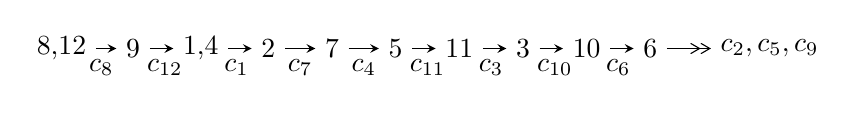
\begin{tikzpicture}[x=23pt, y=7pt]
	% node
	\node (A0) at (-1/8, 0) {8,12};
	\node (A1) at (1, 0) {9};
	\node (A2) at (33/16, 0) {1,4};
	\node (A3) at (25/8, 0) {2};
	\node (A4) at (33/8, 0) {7};
	\node (A5) at (41/8, 0) {5};
	\node (A6) at (49/8, 0) {11};
	\node (A7) at (57/8, 0) {3};
	\node (A8) at (65/8, 0) {10};
	\node (A9) at (73/8, 0) {6};
	\node (C1) at (1/2, -1) {$c_{8}$};
	\node (C2) at (3/2, -1) {$c_{12}$};
	\node (C3) at (21/8, -1) {$c_{1}$};
	\node (C4) at (29/8, -1) {$c_{7}$};
	\node (C5) at (37/8, -1) {$c_{4}$};
	\node (C6) at (45/8, -1) {$c_{11}$};
	\node (C7) at (53/8, -1) {$c_{3}$};
	\node (C8) at (61/8, -1) {$c_{10}$};
	\node (C9) at (69/8, -1) {$c_{6}$};
	\node (A10) at (11, 0) {$c_{2},c_{5},c_{9}$};

	% edge
	\draw[->,>=stealth]	
	(A0) edge (A1) (A1) edge (A2) (A2) edge (A3) (A3) edge (A4) (A4) edge (A5) (A5) edge (A6) (A6) edge (A7) (A7) edge (A8) (A8) edge (A9) ;
	\draw[->>,>={angle 60}]	
	(A9) edge (A10);
\end{tikzpicture} \\ 

\end{tabular} \\

\footnotetext{
The image of knot diagram is generated by the software ``\textbf{Draw programme}" developed by Andrew Bartholomew(\url{http://www.layer8.co.uk/maths/draw/index.htm\#Running-draw}), where we modified some parts for our purpose(\url{https://github.com/CATsTAILs/LinksPainter}).
}\phantom \\ \newline 
\centering \textbf{Ideals for irreducible components\footnotemark of $X_{\text{par}}$} 
 
\begin{align*}
I^u_{1}&=\langle 
164445056849340 u^{52}+1528500349483699 u^{51}+\cdots+224970979095817 b-3074775125088731,\\
\phantom{I^u_{1}}&\phantom{= \langle  }-1.18394\times10^{14} u^{52}-1.52783\times10^{15} u^{51}+\cdots+2.24971\times10^{15} a+4.96511\times10^{16},\\
\phantom{I^u_{1}}&\phantom{= \langle  }u^{53}+8 u^{52}+\cdots-90 u-10\rangle \\
I^u_{2}&=\langle 
u^{27} a- u^{28}+\cdots+b- a,\;2 u^{28}-9 u^{27}+\cdots- a-3,\;u^{29}-5 u^{28}+\cdots+3 u-1\rangle \\
I^u_{3}&=\langle 
- u^{22}+4 u^{21}+\cdots+b+3,\;3 u^{22}-15 u^{21}+\cdots+2 a+13,\;u^{23}-5 u^{22}+\cdots+15 u-2\rangle \\
\\
\end{align*}
\raggedright * 3 irreducible components of $\dim_{\mathbb{C}}=0$, with total 134 representations.\\
\footnotetext{All coefficients of polynomials are rational numbers. But the coefficients are sometimes approximated in decimal forms when there is not enough margin.}
\newpage
\renewcommand{\arraystretch}{1}
\centering \section*{I. $I^u_{1}= \langle 1.64\times10^{14} u^{52}+1.53\times10^{15} u^{51}+\cdots+2.25\times10^{14} b-3.07\times10^{15},\;-1.18\times10^{14} u^{52}-1.53\times10^{15} u^{51}+\cdots+2.25\times10^{15} a+4.97\times10^{16},\;u^{53}+8 u^{52}+\cdots-90 u-10 \rangle$}
\flushleft \textbf{(i) Arc colorings}\\
\begin{tabular}{m{7pt} m{180pt} m{7pt} m{180pt} }
\flushright $a_{8}=$&$\begin{pmatrix}1\\0\end{pmatrix}$ \\
\flushright $a_{12}=$&$\begin{pmatrix}0\\u\end{pmatrix}$ \\
\flushright $a_{9}=$&$\begin{pmatrix}1\\u^2\end{pmatrix}$ \\
\flushright $a_{1}=$&$\begin{pmatrix}- u\\u\end{pmatrix}$ \\
\flushright $a_{4}=$&$\begin{pmatrix}0.0526262 u^{52}+0.679123 u^{51}+\cdots-152.718 u-22.0700\\-0.730961 u^{52}-6.79421 u^{51}+\cdots+138.193 u+13.6674\end{pmatrix}$ \\
\flushright $a_{2}=$&$\begin{pmatrix}0.951306 u^{52}+5.67430 u^{51}+\cdots+62.4823 u+6.08672\\0.0348007 u^{52}+1.25907 u^{51}+\cdots-17.3975 u-0.306208\end{pmatrix}$ \\
\flushright $a_{7}=$&$\begin{pmatrix}u^2+1\\- u^2\end{pmatrix}$ \\
\flushright $a_{5}=$&$\begin{pmatrix}-1.10863 u^{52}-7.59814 u^{51}+\cdots-101.312 u-14.6597\\-0.258114 u^{52}-2.60484 u^{51}+\cdots+17.3337 u-0.526262\end{pmatrix}$ \\
\flushright $a_{11}=$&$\begin{pmatrix}u\\u^3+u\end{pmatrix}$ \\
\flushright $a_{3}=$&$\begin{pmatrix}0.607936 u^{52}+5.21530 u^{51}+\cdots-182.592 u-23.9187\\-0.681469 u^{52}-6.43444 u^{51}+\cdots+122.305 u+12.7557\end{pmatrix}$ \\
\flushright $a_{10}=$&$\begin{pmatrix}0.136819 u^{52}+0.281235 u^{51}+\cdots-6.32329 u-1.45857\\0.651638 u^{52}+6.44090 u^{51}+\cdots-60.8623 u-7.32736\end{pmatrix}$ \\
\flushright $a_{6}=$&$\begin{pmatrix}-0.202862 u^{52}-1.47817 u^{51}+\cdots-33.2032 u-1.30412\\-0.528097 u^{52}-4.04273 u^{51}+\cdots-8.57804 u-2.01689\end{pmatrix}$\\&\end{tabular}
\flushleft \textbf{(ii) Obstruction class $= -1$}\\~\\
\flushleft \textbf{(iii) Cusp Shapes $= -\frac{1416175396984759}{224970979095817} u^{52}-\frac{11695896348510825}{224970979095817} u^{51}+\cdots+\frac{110459786772108940}{224970979095817} u+\frac{4937112965853666}{224970979095817}$}\\~\\
\newpage\renewcommand{\arraystretch}{1}
\flushleft \textbf{(iv) u-Polynomials at the component}\newline \\
\begin{tabular}{m{50pt}|m{274pt}}
Crossings & \hspace{64pt}u-Polynomials at each crossing \\
\hline $$\begin{aligned}c_{1},c_{4}\end{aligned}$$&$\begin{aligned}
&u^{53}- u^{52}+\cdots+11 u+1
\end{aligned}$\\
\hline $$\begin{aligned}c_{2},c_{5}\end{aligned}$$&$\begin{aligned}
&u^{53}-14 u^{52}+\cdots-604 u+58
\end{aligned}$\\
\hline $$\begin{aligned}c_{3},c_{9}\end{aligned}$$&$\begin{aligned}
&u^{53}- u^{52}+\cdots+76 u+79
\end{aligned}$\\
\hline $$\begin{aligned}c_{6},c_{10}\end{aligned}$$&$\begin{aligned}
&u^{53}+u^{52}+\cdots+5 u+1
\end{aligned}$\\
\hline $$\begin{aligned}c_{7},c_{8},c_{11}\\c_{12}\end{aligned}$$&$\begin{aligned}
&u^{53}-8 u^{52}+\cdots-90 u+10
\end{aligned}$\\
\hline
\end{tabular}\\~\\
\newpage\renewcommand{\arraystretch}{1}
\flushleft \textbf{(v) Riley Polynomials at the component}\newline \\
\begin{tabular}{m{50pt}|m{274pt}}
Crossings & \hspace{64pt}Riley Polynomials at each crossing \\
\hline $$\begin{aligned}c_{1},c_{4}\end{aligned}$$&$\begin{aligned}
&y^{53}+37 y^{52}+\cdots-71 y-1
\end{aligned}$\\
\hline $$\begin{aligned}c_{2},c_{5}\end{aligned}$$&$\begin{aligned}
&y^{53}+30 y^{52}+\cdots+4636 y-3364
\end{aligned}$\\
\hline $$\begin{aligned}c_{3},c_{9}\end{aligned}$$&$\begin{aligned}
&y^{53}+9 y^{52}+\cdots-51894 y-6241
\end{aligned}$\\
\hline $$\begin{aligned}c_{6},c_{10}\end{aligned}$$&$\begin{aligned}
&y^{53}+31 y^{52}+\cdots-87 y-1
\end{aligned}$\\
\hline $$\begin{aligned}c_{7},c_{8},c_{11}\\c_{12}\end{aligned}$$&$\begin{aligned}
&y^{53}+64 y^{52}+\cdots-1080 y-100
\end{aligned}$\\
\hline
\end{tabular}\\~\\
\newpage\flushleft \textbf{(vi) Complex Volumes and Cusp Shapes}
$$\begin{array}{c|c|c}  
\text{Solutions to }I^u_{1}& \I (\text{vol} + \sqrt{-1}CS) & \text{Cusp shape}\\
 \hline 
\begin{aligned}
u &= -0.571488 + 0.854314 I \\
a &= \phantom{-}0.032566 - 0.185130 I \\
b &= \phantom{-}1.47379 + 0.14025 I\end{aligned}
 & \phantom{-}6.0412 + 14.8317 I & \phantom{-0.000000 } 0 \\ \hline\begin{aligned}
u &= -0.571488 - 0.854314 I \\
a &= \phantom{-}0.032566 + 0.185130 I \\
b &= \phantom{-}1.47379 - 0.14025 I\end{aligned}
 & \phantom{-}6.0412 - 14.8317 I & \phantom{-0.000000 } 0 \\ \hline\begin{aligned}
u &= -0.333373 + 0.893716 I \\
a &= \phantom{-}0.122196 + 0.270454 I \\
b &= \phantom{-}0.752660 - 0.742316 I\end{aligned}
 & \phantom{-}3.25780 - 1.48286 I & \phantom{-0.000000 } 0 \\ \hline\begin{aligned}
u &= -0.333373 - 0.893716 I \\
a &= \phantom{-}0.122196 - 0.270454 I \\
b &= \phantom{-}0.752660 + 0.742316 I\end{aligned}
 & \phantom{-}3.25780 + 1.48286 I & \phantom{-0.000000 } 0 \\ \hline\begin{aligned}
u &= -0.514882 + 0.797117 I \\
a &= -0.190321 + 0.041120 I \\
b &= -1.47025 - 0.02613 I\end{aligned}
 & \phantom{-}2.18355 + 8.95648 I & \phantom{-0.000000 } 0 \\ \hline\begin{aligned}
u &= -0.514882 - 0.797117 I \\
a &= -0.190321 - 0.041120 I \\
b &= -1.47025 + 0.02613 I\end{aligned}
 & \phantom{-}2.18355 - 8.95648 I & \phantom{-0.000000 } 0 \\ \hline\begin{aligned}
u &= -0.361910 + 0.832045 I \\
a &= \phantom{-}0.048979 + 0.404557 I \\
b &= \phantom{-}1.59883 - 0.06719 I\end{aligned}
 & \phantom{-}7.41008 + 3.50903 I & \phantom{-0.000000 } 0 \\ \hline\begin{aligned}
u &= -0.361910 - 0.832045 I \\
a &= \phantom{-}0.048979 - 0.404557 I \\
b &= \phantom{-}1.59883 + 0.06719 I\end{aligned}
 & \phantom{-}7.41008 - 3.50903 I & \phantom{-0.000000 } 0 \\ \hline\begin{aligned}
u &= -0.533035 + 0.701728 I \\
a &= -0.185867 + 0.304202 I \\
b &= -0.714550 + 0.710437 I\end{aligned}
 & \phantom{-}6.11438 + 3.16811 I & \phantom{-0.000000 } 0 \\ \hline\begin{aligned}
u &= -0.533035 - 0.701728 I \\
a &= -0.185867 - 0.304202 I \\
b &= -0.714550 - 0.710437 I\end{aligned}
 & \phantom{-}6.11438 - 3.16811 I & \phantom{-0.000000 } 0\\
 \hline 
 \end{array}$$\newpage$$\begin{array}{c|c|c}  
\text{Solutions to }I^u_{1}& \I (\text{vol} + \sqrt{-1}CS) & \text{Cusp shape}\\
 \hline 
\begin{aligned}
u &= -0.508757 + 1.013150 I \\
a &= \phantom{-}0.189315 - 0.149873 I \\
b &= -0.836774 + 0.733674 I\end{aligned}
 & \phantom{-}6.93290 - 5.87882 I & \phantom{-0.000000 } 0 \\ \hline\begin{aligned}
u &= -0.508757 - 1.013150 I \\
a &= \phantom{-}0.189315 + 0.149873 I \\
b &= -0.836774 - 0.733674 I\end{aligned}
 & \phantom{-}6.93290 + 5.87882 I & \phantom{-0.000000 } 0 \\ \hline\begin{aligned}
u &= -0.792218 + 0.065716 I \\
a &= \phantom{-}0.613499 + 1.156200 I \\
b &= \phantom{-}0.058973 + 0.266092 I\end{aligned}
 & \phantom{-}3.65102 - 10.30440 I & -8.91398 + 7.10436 I \\ \hline\begin{aligned}
u &= -0.792218 - 0.065716 I \\
a &= \phantom{-}0.613499 - 1.156200 I \\
b &= \phantom{-}0.058973 - 0.266092 I\end{aligned}
 & \phantom{-}3.65102 + 10.30440 I & -8.91398 - 7.10436 I \\ \hline\begin{aligned}
u &= \phantom{-}0.146692 + 1.220860 I \\
a &= \phantom{-}0.051603 + 0.425034 I \\
b &= \phantom{-}0.200402 - 0.509149 I\end{aligned}
 & \phantom{-}2.65741 - 1.99035 I & \phantom{-0.000000 } 0 \\ \hline\begin{aligned}
u &= \phantom{-}0.146692 - 1.220860 I \\
a &= \phantom{-}0.051603 - 0.425034 I \\
b &= \phantom{-}0.200402 + 0.509149 I\end{aligned}
 & \phantom{-}2.65741 + 1.99035 I & \phantom{-0.000000 } 0 \\ \hline\begin{aligned}
u &= \phantom{-}0.362018 + 0.677893 I \\
a &= -0.245195 + 0.777289 I \\
b &= \phantom{-}0.514294 - 0.329515 I\end{aligned}
 & \phantom{-}1.50207 - 2.55064 I & -9.75941 + 4.81296 I \\ \hline\begin{aligned}
u &= \phantom{-}0.362018 - 0.677893 I \\
a &= -0.245195 - 0.777289 I \\
b &= \phantom{-}0.514294 + 0.329515 I\end{aligned}
 & \phantom{-}1.50207 + 2.55064 I & -9.75941 - 4.81296 I \\ \hline\begin{aligned}
u &= \phantom{-}0.690789 + 0.151095 I \\
a &= \phantom{-}0.180428 - 0.506714 I \\
b &= -0.137160 + 0.263242 I\end{aligned}
 & -0.340350 - 0.823156 I & -15.6364 + 2.5706 I \\ \hline\begin{aligned}
u &= \phantom{-}0.690789 - 0.151095 I \\
a &= \phantom{-}0.180428 + 0.506714 I \\
b &= -0.137160 - 0.263242 I\end{aligned}
 & -0.340350 + 0.823156 I & -15.6364 - 2.5706 I\\
 \hline 
 \end{array}$$\newpage$$\begin{array}{c|c|c}  
\text{Solutions to }I^u_{1}& \I (\text{vol} + \sqrt{-1}CS) & \text{Cusp shape}\\
 \hline 
\begin{aligned}
u &= \phantom{-}0.084709 + 0.684083 I \\
a &= -0.34764 - 1.68310 I \\
b &= -1.17130 + 0.93302 I\end{aligned}
 & \phantom{-}4.62340 - 0.33572 I & -1.95908 - 0.70589 I \\ \hline\begin{aligned}
u &= \phantom{-}0.084709 - 0.684083 I \\
a &= -0.34764 + 1.68310 I \\
b &= -1.17130 - 0.93302 I\end{aligned}
 & \phantom{-}4.62340 + 0.33572 I & -1.95908 + 0.70589 I \\ \hline\begin{aligned}
u &= -0.679848 + 0.096270 I \\
a &= -0.595374 - 1.265890 I \\
b &= -0.100020 - 0.402728 I\end{aligned}
 & \phantom{-}0.07833 - 4.93869 I & -12.17317 + 4.95425 I \\ \hline\begin{aligned}
u &= -0.679848 - 0.096270 I \\
a &= -0.595374 + 1.265890 I \\
b &= -0.100020 + 0.402728 I\end{aligned}
 & \phantom{-}0.07833 + 4.93869 I & -12.17317 - 4.95425 I \\ \hline\begin{aligned}
u &= \phantom{-}0.331739 + 1.322100 I \\
a &= \phantom{-}0.345446 - 0.293824 I \\
b &= -0.497956 + 0.157982 I\end{aligned}
 & \phantom{-}4.28652 - 4.55905 I & \phantom{-0.000000 } 0 \\ \hline\begin{aligned}
u &= \phantom{-}0.331739 - 1.322100 I \\
a &= \phantom{-}0.345446 + 0.293824 I \\
b &= -0.497956 - 0.157982 I\end{aligned}
 & \phantom{-}4.28652 + 4.55905 I & \phantom{-0.000000 } 0 \\ \hline\begin{aligned}
u &= -0.548171 + 0.130924 I \\
a &= \phantom{-}0.97680 - 1.21375 I \\
b &= \phantom{-}0.379782 - 0.413933 I\end{aligned}
 & \phantom{-}4.58827 + 0.51390 I & -6.27299 - 1.69527 I \\ \hline\begin{aligned}
u &= -0.548171 - 0.130924 I \\
a &= \phantom{-}0.97680 + 1.21375 I \\
b &= \phantom{-}0.379782 + 0.413933 I\end{aligned}
 & \phantom{-}4.58827 - 0.51390 I & -6.27299 + 1.69527 I \\ \hline\begin{aligned}
u &= -0.193987 + 0.484551 I \\
a &= -0.23294 - 1.53315 I \\
b &= -1.067610 - 0.351475 I\end{aligned}
 & -1.41579 + 0.84257 I & -19.4951 - 7.3381 I \\ \hline\begin{aligned}
u &= -0.193987 - 0.484551 I \\
a &= -0.23294 + 1.53315 I \\
b &= -1.067610 + 0.351475 I\end{aligned}
 & -1.41579 - 0.84257 I & -19.4951 + 7.3381 I\\
 \hline 
 \end{array}$$\newpage$$\begin{array}{c|c|c}  
\text{Solutions to }I^u_{1}& \I (\text{vol} + \sqrt{-1}CS) & \text{Cusp shape}\\
 \hline 
\begin{aligned}
u &= -0.014741 + 0.472127 I \\
a &= \phantom{-}1.57493 + 1.38924 I \\
b &= \phantom{-}0.746773 - 0.962501 I\end{aligned}
 & \phantom{-}3.83390 - 0.06012 I & -2.56930 - 0.12602 I \\ \hline\begin{aligned}
u &= -0.014741 - 0.472127 I \\
a &= \phantom{-}1.57493 - 1.38924 I \\
b &= \phantom{-}0.746773 + 0.962501 I\end{aligned}
 & \phantom{-}3.83390 + 0.06012 I & -2.56930 + 0.12602 I \\ \hline\begin{aligned}
u &= -0.02782 + 1.57717 I \\
a &= \phantom{-}1.95052 + 0.55742 I \\
b &= -2.42122 - 1.38838 I\end{aligned}
 & \phantom{-}5.78164 + 1.46731 I & \phantom{-0.000000 } 0 \\ \hline\begin{aligned}
u &= -0.02782 - 1.57717 I \\
a &= \phantom{-}1.95052 - 0.55742 I \\
b &= -2.42122 + 1.38838 I\end{aligned}
 & \phantom{-}5.78164 - 1.46731 I & \phantom{-0.000000 } 0 \\ \hline\begin{aligned}
u &= -0.01993 + 1.59734 I \\
a &= -1.79395 + 0.64309 I \\
b &= \phantom{-}2.58325 - 0.28191 I\end{aligned}
 & \phantom{-}11.20290 + 0.20541 I & \phantom{-0.000000 } 0 \\ \hline\begin{aligned}
u &= -0.01993 - 1.59734 I \\
a &= -1.79395 - 0.64309 I \\
b &= \phantom{-}2.58325 + 0.28191 I\end{aligned}
 & \phantom{-}11.20290 - 0.20541 I & \phantom{-0.000000 } 0 \\ \hline\begin{aligned}
u &= \phantom{-}0.07759 + 1.59910 I \\
a &= -1.243800 - 0.046636 I \\
b &= \phantom{-}1.55661 + 0.47044 I\end{aligned}
 & \phantom{-}9.25697 - 4.06418 I & \phantom{-0.000000 } 0 \\ \hline\begin{aligned}
u &= \phantom{-}0.07759 - 1.59910 I \\
a &= -1.243800 + 0.046636 I \\
b &= \phantom{-}1.55661 - 0.47044 I\end{aligned}
 & \phantom{-}9.25697 + 4.06418 I & \phantom{-0.000000 } 0 \\ \hline\begin{aligned}
u &= -0.16941 + 1.61795 I \\
a &= \phantom{-}1.35369 - 0.99049 I \\
b &= -2.16566 + 1.05980 I\end{aligned}
 & \phantom{-}13.9905 + 5.8535 I & \phantom{-0.000000 } 0 \\ \hline\begin{aligned}
u &= -0.16941 - 1.61795 I \\
a &= \phantom{-}1.35369 + 0.99049 I \\
b &= -2.16566 - 1.05980 I\end{aligned}
 & \phantom{-}13.9905 - 5.8535 I & \phantom{-0.000000 } 0\\
 \hline 
 \end{array}$$\newpage$$\begin{array}{c|c|c}  
\text{Solutions to }I^u_{1}& \I (\text{vol} + \sqrt{-1}CS) & \text{Cusp shape}\\
 \hline 
\begin{aligned}
u &= \phantom{-}0.02664 + 1.62849 I \\
a &= \phantom{-}2.05682 - 0.56120 I \\
b &= -2.82798 + 0.09247 I\end{aligned}
 & \phantom{-}12.75440 - 0.77114 I & \phantom{-0.000000 } 0 \\ \hline\begin{aligned}
u &= \phantom{-}0.02664 - 1.62849 I \\
a &= \phantom{-}2.05682 + 0.56120 I \\
b &= -2.82798 - 0.09247 I\end{aligned}
 & \phantom{-}12.75440 + 0.77114 I & \phantom{-0.000000 } 0 \\ \hline\begin{aligned}
u &= -0.09741 + 1.63542 I \\
a &= -1.54132 + 0.75143 I \\
b &= \phantom{-}2.30697 - 0.60574 I\end{aligned}
 & \phantom{-}11.84370 + 0.11908 I & \phantom{-0.000000 } 0 \\ \hline\begin{aligned}
u &= -0.09741 - 1.63542 I \\
a &= -1.54132 - 0.75143 I \\
b &= \phantom{-}2.30697 + 0.60574 I\end{aligned}
 & \phantom{-}11.84370 - 0.11908 I & \phantom{-0.000000 } 0 \\ \hline\begin{aligned}
u &= -0.14856 + 1.64246 I \\
a &= \phantom{-}2.41249 - 0.23895 I \\
b &= -3.41599 - 0.26515 I\end{aligned}
 & \phantom{-}10.5226 + 11.4856 I & \phantom{-0.000000 } 0 \\ \hline\begin{aligned}
u &= -0.14856 - 1.64246 I \\
a &= \phantom{-}2.41249 + 0.23895 I \\
b &= -3.41599 + 0.26515 I\end{aligned}
 & \phantom{-}10.5226 - 11.4856 I & \phantom{-0.000000 } 0 \\ \hline\begin{aligned}
u &= -0.10034 + 1.64902 I \\
a &= -2.48542 + 0.14164 I \\
b &= \phantom{-}3.42004 + 0.46088 I\end{aligned}
 & \phantom{-}15.9769 + 5.2810 I & \phantom{-0.000000 } 0 \\ \hline\begin{aligned}
u &= -0.10034 - 1.64902 I \\
a &= -2.48542 - 0.14164 I \\
b &= \phantom{-}3.42004 - 0.46088 I\end{aligned}
 & \phantom{-}15.9769 - 5.2810 I & \phantom{-0.000000 } 0 \\ \hline\begin{aligned}
u &= \phantom{-}0.329619\phantom{ +0.000000I} \\
a &= \phantom{-}0.926533\phantom{ +0.000000I} \\
b &= -0.282332\phantom{ +0.000000I}\end{aligned}
 & -0.644263\phantom{ +0.000000I} & -15.7010\phantom{ +0.000000I} \\ \hline\begin{aligned}
u &= -0.16800 + 1.66325 I \\
a &= -2.36636 + 0.17556 I \\
b &= \phantom{-}3.33573 + 0.29398 I\end{aligned}
 & \phantom{-}14.6437 + 17.6986 I & \phantom{-0.000000 } 0\\
 \hline 
 \end{array}$$\newpage$$\begin{array}{c|c|c}  
\text{Solutions to }I^u_{1}& \I (\text{vol} + \sqrt{-1}CS) & \text{Cusp shape}\\
 \hline 
\begin{aligned}
u &= -0.16800 - 1.66325 I \\
a &= -2.36636 - 0.17556 I \\
b &= \phantom{-}3.33573 - 0.29398 I\end{aligned}
 & \phantom{-}14.6437 - 17.6986 I & \phantom{-0.000000 } 0 \\ \hline\begin{aligned}
u &= -0.10112 + 1.71662 I \\
a &= \phantom{-}1.35564 - 0.64503 I \\
b &= -1.96049 + 0.55509 I\end{aligned}
 & \phantom{-}16.5969 - 3.5463 I & \phantom{-0.000000 } 0 \\ \hline\begin{aligned}
u &= -0.10112 - 1.71662 I \\
a &= \phantom{-}1.35564 + 0.64503 I \\
b &= -1.96049 - 0.55509 I\end{aligned}
 & \phantom{-}16.5969 + 3.5463 I & \phantom{-0.000000 } 0\\
 \hline 
 \end{array}$$\newpage\newpage\renewcommand{\arraystretch}{1}
\centering \section*{II. $I^u_{2}= \langle u^{27} a- u^{28}+\cdots+b- a,\;2 u^{28}-9 u^{27}+\cdots- a-3,\;u^{29}-5 u^{28}+\cdots+3 u-1 \rangle$}
\flushleft \textbf{(i) Arc colorings}\\
\begin{tabular}{m{7pt} m{180pt} m{7pt} m{180pt} }
\flushright $a_{8}=$&$\begin{pmatrix}1\\0\end{pmatrix}$ \\
\flushright $a_{12}=$&$\begin{pmatrix}0\\u\end{pmatrix}$ \\
\flushright $a_{9}=$&$\begin{pmatrix}1\\u^2\end{pmatrix}$ \\
\flushright $a_{1}=$&$\begin{pmatrix}- u\\u\end{pmatrix}$ \\
\flushright $a_{4}=$&$\begin{pmatrix}a\\- u^{27} a+u^{28}+\cdots+a-2 u\end{pmatrix}$ \\
\flushright $a_{2}=$&$\begin{pmatrix}u^{28} a-5 u^{27} a+\cdots-8 u+2\\u^{26} a+u^{27}+\cdots- a u+3 u\end{pmatrix}$ \\
\flushright $a_{7}=$&$\begin{pmatrix}u^2+1\\- u^2\end{pmatrix}$ \\
\flushright $a_{5}=$&$\begin{pmatrix}u^{28} a-5 u^{27} a+\cdots-4 a u+2 a\\- u^{27}+6 u^{26}+\cdots+a u- u\end{pmatrix}$ \\
\flushright $a_{11}=$&$\begin{pmatrix}u\\u^3+u\end{pmatrix}$ \\
\flushright $a_{3}=$&$\begin{pmatrix}- u^{28} a+5 u^{27} a+\cdots+3 a u+u\\- u^{27}+6 u^{26}+\cdots+a u- u\end{pmatrix}$ \\
\flushright $a_{10}=$&$\begin{pmatrix}u^{28} a-5 u^{27} a+\cdots+2 a-2\\u^{27}-4 u^{26}+\cdots- a u+3 u\end{pmatrix}$ \\
\flushright $a_{6}=$&$\begin{pmatrix}u^{28} a-5 u^{27} a+\cdots+2 a+1\\u^{27}-6 u^{26}+\cdots+a u-7 u^2\end{pmatrix}$\\&\end{tabular}
\flushleft \textbf{(ii) Obstruction class $= -1$}\\~\\
\flushleft \textbf{(iii) Cusp Shapes $= -4 u^{27}+20 u^{26}-116 u^{25}+400 u^{24}-1332 u^{23}+3464 u^{22}-8320 u^{21}+17056 u^{20}-31872 u^{19}+52660 u^{18}-78908 u^{17}+105992 u^{16}-128548 u^{15}+140200 u^{14}-137200 u^{13}+120424 u^{12}-94128 u^{11}+65704 u^{10}-40668 u^9+22460 u^8-11040 u^7+4780 u^6-1836 u^5+588 u^4-192 u^3+60 u^2-16 u-10$}\\~\\
\newpage\renewcommand{\arraystretch}{1}
\flushleft \textbf{(iv) u-Polynomials at the component}\newline \\
\begin{tabular}{m{50pt}|m{274pt}}
Crossings & \hspace{64pt}u-Polynomials at each crossing \\
\hline $$\begin{aligned}c_{1},c_{4}\end{aligned}$$&$\begin{aligned}
&u^{58}-9 u^{57}+\cdots-630 u+229
\end{aligned}$\\
\hline $$\begin{aligned}c_{2},c_{5}\end{aligned}$$&$\begin{aligned}
&(u^{29}+9 u^{28}+\cdots+5 u+1)^{2}
\end{aligned}$\\
\hline $$\begin{aligned}c_{3},c_{9}\end{aligned}$$&$\begin{aligned}
&u^{58}- u^{57}+\cdots+1134 u+197
\end{aligned}$\\
\hline $$\begin{aligned}c_{6},c_{10}\end{aligned}$$&$\begin{aligned}
&u^{58}+5 u^{57}+\cdots+4 u+1
\end{aligned}$\\
\hline $$\begin{aligned}c_{7},c_{8},c_{11}\\c_{12}\end{aligned}$$&$\begin{aligned}
&(u^{29}+5 u^{28}+\cdots+3 u+1)^{2}
\end{aligned}$\\
\hline
\end{tabular}\\~\\
\newpage\renewcommand{\arraystretch}{1}
\flushleft \textbf{(v) Riley Polynomials at the component}\newline \\
\begin{tabular}{m{50pt}|m{274pt}}
Crossings & \hspace{64pt}Riley Polynomials at each crossing \\
\hline $$\begin{aligned}c_{1},c_{4}\end{aligned}$$&$\begin{aligned}
&y^{58}-5 y^{57}+\cdots+1349912 y+52441
\end{aligned}$\\
\hline $$\begin{aligned}c_{2},c_{5}\end{aligned}$$&$\begin{aligned}
&(y^{29}+19 y^{28}+\cdots-13 y-1)^{2}
\end{aligned}$\\
\hline $$\begin{aligned}c_{3},c_{9}\end{aligned}$$&$\begin{aligned}
&y^{58}+19 y^{57}+\cdots-508200 y+38809
\end{aligned}$\\
\hline $$\begin{aligned}c_{6},c_{10}\end{aligned}$$&$\begin{aligned}
&y^{58}-9 y^{57}+\cdots-12 y+1
\end{aligned}$\\
\hline $$\begin{aligned}c_{7},c_{8},c_{11}\\c_{12}\end{aligned}$$&$\begin{aligned}
&(y^{29}+35 y^{28}+\cdots-13 y-1)^{2}
\end{aligned}$\\
\hline
\end{tabular}\\~\\
\newpage\flushleft \textbf{(vi) Complex Volumes and Cusp Shapes}
$$\begin{array}{c|c|c}  
\text{Solutions to }I^u_{2}& \I (\text{vol} + \sqrt{-1}CS) & \text{Cusp shape}\\
 \hline 
\begin{aligned}
u &= \phantom{-}0.195688 + 0.954423 I \\
a &= -0.972128 - 0.906034 I \\
b &= \phantom{-}1.76849 + 0.94660 I\end{aligned}
 & \phantom{-}6.38732 - 5.06785 I & \phantom{-}0.07562 + 6.89681 I \\ \hline\begin{aligned}
u &= \phantom{-}0.195688 + 0.954423 I \\
a &= -0.369914 + 0.336353 I \\
b &= -1.063590 + 0.478683 I\end{aligned}
 & \phantom{-}6.38732 - 5.06785 I & \phantom{-}0.07562 + 6.89681 I \\ \hline\begin{aligned}
u &= \phantom{-}0.195688 - 0.954423 I \\
a &= -0.972128 + 0.906034 I \\
b &= \phantom{-}1.76849 - 0.94660 I\end{aligned}
 & \phantom{-}6.38732 + 5.06785 I & \phantom{-}0.07562 - 6.89681 I \\ \hline\begin{aligned}
u &= \phantom{-}0.195688 - 0.954423 I \\
a &= -0.369914 - 0.336353 I \\
b &= -1.063590 - 0.478683 I\end{aligned}
 & \phantom{-}6.38732 + 5.06785 I & \phantom{-}0.07562 - 6.89681 I \\ \hline\begin{aligned}
u &= \phantom{-}0.501023 + 0.778198 I \\
a &= \phantom{-}0.130975 + 0.416319 I \\
b &= \phantom{-}1.072090 - 0.191134 I\end{aligned}
 & \phantom{-}1.64148 - 3.39274 I & -11.48736 + 3.20502 I \\ \hline\begin{aligned}
u &= \phantom{-}0.501023 + 0.778198 I \\
a &= -0.169674 + 0.385781 I \\
b &= -0.711264 - 0.349089 I\end{aligned}
 & \phantom{-}1.64148 - 3.39274 I & -11.48736 + 3.20502 I \\ \hline\begin{aligned}
u &= \phantom{-}0.501023 - 0.778198 I \\
a &= \phantom{-}0.130975 - 0.416319 I \\
b &= \phantom{-}1.072090 + 0.191134 I\end{aligned}
 & \phantom{-}1.64148 + 3.39274 I & -11.48736 - 3.20502 I \\ \hline\begin{aligned}
u &= \phantom{-}0.501023 - 0.778198 I \\
a &= -0.169674 - 0.385781 I \\
b &= -0.711264 + 0.349089 I\end{aligned}
 & \phantom{-}1.64148 + 3.39274 I & -11.48736 - 3.20502 I \\ \hline\begin{aligned}
u &= \phantom{-}0.566469 + 0.934578 I \\
a &= \phantom{-}0.467515 - 0.263005 I \\
b &= -1.364860 + 0.113870 I\end{aligned}
 & \phantom{-}2.84920 - 5.41618 I & -8.6789 + 12.8683 I \\ \hline\begin{aligned}
u &= \phantom{-}0.566469 + 0.934578 I \\
a &= \phantom{-}0.256548 - 0.030398 I \\
b &= \phantom{-}0.670641 - 0.168517 I\end{aligned}
 & \phantom{-}2.84920 - 5.41618 I & -8.6789 + 12.8683 I\\
 \hline 
 \end{array}$$\newpage$$\begin{array}{c|c|c}  
\text{Solutions to }I^u_{2}& \I (\text{vol} + \sqrt{-1}CS) & \text{Cusp shape}\\
 \hline 
\begin{aligned}
u &= \phantom{-}0.566469 - 0.934578 I \\
a &= \phantom{-}0.467515 + 0.263005 I \\
b &= -1.364860 - 0.113870 I\end{aligned}
 & \phantom{-}2.84920 + 5.41618 I & -8.6789 - 12.8683 I \\ \hline\begin{aligned}
u &= \phantom{-}0.566469 - 0.934578 I \\
a &= \phantom{-}0.256548 + 0.030398 I \\
b &= \phantom{-}0.670641 + 0.168517 I\end{aligned}
 & \phantom{-}2.84920 + 5.41618 I & -8.6789 - 12.8683 I \\ \hline\begin{aligned}
u &= \phantom{-}0.786511 + 0.103322 I \\
a &= \phantom{-}0.075590 - 0.942723 I \\
b &= -0.203314 + 0.156273 I\end{aligned}
 & -0.273694 - 0.889339 I & -18.0678 + 6.3049 I \\ \hline\begin{aligned}
u &= \phantom{-}0.786511 + 0.103322 I \\
a &= \phantom{-}0.313505 + 0.056568 I \\
b &= -0.065851 + 0.346476 I\end{aligned}
 & -0.273694 - 0.889339 I & -18.0678 + 6.3049 I \\ \hline\begin{aligned}
u &= \phantom{-}0.786511 - 0.103322 I \\
a &= \phantom{-}0.075590 + 0.942723 I \\
b &= -0.203314 - 0.156273 I\end{aligned}
 & -0.273694 + 0.889339 I & -18.0678 - 6.3049 I \\ \hline\begin{aligned}
u &= \phantom{-}0.786511 - 0.103322 I \\
a &= \phantom{-}0.313505 - 0.056568 I \\
b &= -0.065851 - 0.346476 I\end{aligned}
 & -0.273694 + 0.889339 I & -18.0678 - 6.3049 I \\ \hline\begin{aligned}
u &= \phantom{-}0.494082 + 0.587228 I \\
a &= \phantom{-}0.302521 + 0.875921 I \\
b &= \phantom{-}0.983777 - 0.141714 I\end{aligned}
 & \phantom{-}1.43997 - 3.32019 I & -12.1625 + 7.9197 I \\ \hline\begin{aligned}
u &= \phantom{-}0.494082 + 0.587228 I \\
a &= -0.583892 + 0.586111 I \\
b &= -0.304504 - 0.604439 I\end{aligned}
 & \phantom{-}1.43997 - 3.32019 I & -12.1625 + 7.9197 I \\ \hline\begin{aligned}
u &= \phantom{-}0.494082 - 0.587228 I \\
a &= \phantom{-}0.302521 - 0.875921 I \\
b &= \phantom{-}0.983777 + 0.141714 I\end{aligned}
 & \phantom{-}1.43997 + 3.32019 I & -12.1625 - 7.9197 I \\ \hline\begin{aligned}
u &= \phantom{-}0.494082 - 0.587228 I \\
a &= -0.583892 - 0.586111 I \\
b &= -0.304504 + 0.604439 I\end{aligned}
 & \phantom{-}1.43997 + 3.32019 I & -12.1625 - 7.9197 I\\
 \hline 
 \end{array}$$\newpage$$\begin{array}{c|c|c}  
\text{Solutions to }I^u_{2}& \I (\text{vol} + \sqrt{-1}CS) & \text{Cusp shape}\\
 \hline 
\begin{aligned}
u &= -0.216772 + 0.623278 I \\
a &= -1.076190 - 0.337838 I \\
b &= \phantom{-}2.01966 + 0.88632 I\end{aligned}
 & \phantom{-}3.13189 + 6.56560 I & -7.1171 - 12.8291 I \\ \hline\begin{aligned}
u &= -0.216772 + 0.623278 I \\
a &= \phantom{-}0.41367 + 2.27782 I \\
b &= -0.130503 + 0.584963 I\end{aligned}
 & \phantom{-}3.13189 + 6.56560 I & -7.1171 - 12.8291 I \\ \hline\begin{aligned}
u &= -0.216772 - 0.623278 I \\
a &= -1.076190 + 0.337838 I \\
b &= \phantom{-}2.01966 - 0.88632 I\end{aligned}
 & \phantom{-}3.13189 - 6.56560 I & -7.1171 + 12.8291 I \\ \hline\begin{aligned}
u &= -0.216772 - 0.623278 I \\
a &= \phantom{-}0.41367 - 2.27782 I \\
b &= -0.130503 - 0.584963 I\end{aligned}
 & \phantom{-}3.13189 - 6.56560 I & -7.1171 + 12.8291 I \\ \hline\begin{aligned}
u &= -0.188616 + 0.478965 I \\
a &= \phantom{-}0.044120 - 1.082270 I \\
b &= -1.256420 - 0.410029 I\end{aligned}
 & -1.41975 + 0.83016 I & -16.3280 - 7.8903 I \\ \hline\begin{aligned}
u &= -0.188616 + 0.478965 I \\
a &= -0.34963 - 1.92596 I \\
b &= -0.746967 - 0.337731 I\end{aligned}
 & -1.41975 + 0.83016 I & -16.3280 - 7.8903 I \\ \hline\begin{aligned}
u &= -0.188616 - 0.478965 I \\
a &= \phantom{-}0.044120 + 1.082270 I \\
b &= -1.256420 + 0.410029 I\end{aligned}
 & -1.41975 - 0.83016 I & -16.3280 + 7.8903 I \\ \hline\begin{aligned}
u &= -0.188616 - 0.478965 I \\
a &= -0.34963 + 1.92596 I \\
b &= -0.746967 + 0.337731 I\end{aligned}
 & -1.41975 - 0.83016 I & -16.3280 + 7.8903 I \\ \hline\begin{aligned}
u &= \phantom{-}0.505604\phantom{ +0.000000I} \\
a &= \phantom{-}0.870038 + 0.975031 I \\
b &= -0.376046 + 0.324956 I\end{aligned}
 & -0.296707\phantom{ +0.000000I} & -14.3160\phantom{ +0.000000I} \\ \hline\begin{aligned}
u &= \phantom{-}0.505604\phantom{ +0.000000I} \\
a &= \phantom{-}0.870038 - 0.975031 I \\
b &= -0.376046 - 0.324956 I\end{aligned}
 & -0.296707\phantom{ +0.000000I} & -14.3160\phantom{ +0.000000I}\\
 \hline 
 \end{array}$$\newpage$$\begin{array}{c|c|c}  
\text{Solutions to }I^u_{2}& \I (\text{vol} + \sqrt{-1}CS) & \text{Cusp shape}\\
 \hline 
\begin{aligned}
u &= \phantom{-}0.04467 + 1.55722 I \\
a &= \phantom{-}0.023319 + 0.830907 I \\
b &= -0.295170 - 0.221687 I\end{aligned}
 & \phantom{-}8.27486 - 4.88057 I & -12.00000 + 5.42301 I \\ \hline\begin{aligned}
u &= \phantom{-}0.04467 + 1.55722 I \\
a &= -2.56750 - 0.54184 I \\
b &= \phantom{-}3.67601 + 0.75264 I\end{aligned}
 & \phantom{-}8.27486 - 4.88057 I & -12.00000 + 5.42301 I \\ \hline\begin{aligned}
u &= \phantom{-}0.04467 - 1.55722 I \\
a &= \phantom{-}0.023319 - 0.830907 I \\
b &= -0.295170 + 0.221687 I\end{aligned}
 & \phantom{-}8.27486 + 4.88057 I & -12.00000 - 5.42301 I \\ \hline\begin{aligned}
u &= \phantom{-}0.04467 - 1.55722 I \\
a &= -2.56750 + 0.54184 I \\
b &= \phantom{-}3.67601 - 0.75264 I\end{aligned}
 & \phantom{-}8.27486 + 4.88057 I & -12.00000 - 5.42301 I \\ \hline\begin{aligned}
u &= -0.02297 + 1.57694 I \\
a &= \phantom{-}1.031300 + 0.891923 I \\
b &= -1.27596 - 1.98763 I\end{aligned}
 & \phantom{-}5.75764 + 1.39775 I & -12.00000 + 0. I\phantom{ +0.000000I} \\ \hline\begin{aligned}
u &= -0.02297 + 1.57694 I \\
a &= \phantom{-}2.42065 + 0.36806 I \\
b &= -2.90576 - 0.83473 I\end{aligned}
 & \phantom{-}5.75764 + 1.39775 I & -12.00000 + 0. I\phantom{ +0.000000I} \\ \hline\begin{aligned}
u &= -0.02297 - 1.57694 I \\
a &= \phantom{-}1.031300 - 0.891923 I \\
b &= -1.27596 + 1.98763 I\end{aligned}
 & \phantom{-}5.75764 - 1.39775 I & -12.00000 + 0. I\phantom{ +0.000000I} \\ \hline\begin{aligned}
u &= -0.02297 - 1.57694 I \\
a &= \phantom{-}2.42065 - 0.36806 I \\
b &= -2.90576 + 0.83473 I\end{aligned}
 & \phantom{-}5.75764 - 1.39775 I & -12.00000 + 0. I\phantom{ +0.000000I} \\ \hline\begin{aligned}
u &= -0.04870 + 1.60940 I \\
a &= \phantom{-}0.30754 - 1.70729 I \\
b &= -0.53659 + 3.24918 I\end{aligned}
 & \phantom{-}10.92340 + 7.47108 I & -12.00000 + 0. I\phantom{ +0.000000I} \\ \hline\begin{aligned}
u &= -0.04870 + 1.60940 I \\
a &= -3.14722 - 0.78581 I \\
b &= \phantom{-}3.59046 + 0.95749 I\end{aligned}
 & \phantom{-}10.92340 + 7.47108 I & -12.00000 + 0. I\phantom{ +0.000000I}\\
 \hline 
 \end{array}$$\newpage$$\begin{array}{c|c|c}  
\text{Solutions to }I^u_{2}& \I (\text{vol} + \sqrt{-1}CS) & \text{Cusp shape}\\
 \hline 
\begin{aligned}
u &= -0.04870 - 1.60940 I \\
a &= \phantom{-}0.30754 + 1.70729 I \\
b &= -0.53659 - 3.24918 I\end{aligned}
 & \phantom{-}10.92340 - 7.47108 I & -12.00000 + 0. I\phantom{ +0.000000I} \\ \hline\begin{aligned}
u &= -0.04870 - 1.60940 I \\
a &= -3.14722 + 0.78581 I \\
b &= \phantom{-}3.59046 - 0.95749 I\end{aligned}
 & \phantom{-}10.92340 - 7.47108 I & -12.00000 + 0. I\phantom{ +0.000000I} \\ \hline\begin{aligned}
u &= -0.243173 + 0.281252 I \\
a &= \phantom{-}2.16112 - 0.32713 I \\
b &= \phantom{-}0.955798 + 0.909043 I\end{aligned}
 & \phantom{-}2.20930 - 4.73918 I & -12.69833 + 0.12567 I \\ \hline\begin{aligned}
u &= -0.243173 + 0.281252 I \\
a &= \phantom{-}0.20097 + 3.38461 I \\
b &= \phantom{-}0.552481 - 0.575987 I\end{aligned}
 & \phantom{-}2.20930 - 4.73918 I & -12.69833 + 0.12567 I \\ \hline\begin{aligned}
u &= -0.243173 - 0.281252 I \\
a &= \phantom{-}2.16112 + 0.32713 I \\
b &= \phantom{-}0.955798 - 0.909043 I\end{aligned}
 & \phantom{-}2.20930 + 4.73918 I & -12.69833 - 0.12567 I \\ \hline\begin{aligned}
u &= -0.243173 - 0.281252 I \\
a &= \phantom{-}0.20097 - 3.38461 I \\
b &= \phantom{-}0.552481 + 0.575987 I\end{aligned}
 & \phantom{-}2.20930 + 4.73918 I & -12.69833 - 0.12567 I \\ \hline\begin{aligned}
u &= \phantom{-}0.14130 + 1.64406 I \\
a &= \phantom{-}1.39862 + 0.38362 I \\
b &= -2.00910 + 0.04697 I\end{aligned}
 & \phantom{-}9.97047 - 5.82183 I & \phantom{-0.000000 } 0 \\ \hline\begin{aligned}
u &= \phantom{-}0.14130 + 1.64406 I \\
a &= -2.13183 - 0.07965 I \\
b &= \phantom{-}3.00192 - 0.19303 I\end{aligned}
 & \phantom{-}9.97047 - 5.82183 I & \phantom{-0.000000 } 0 \\ \hline\begin{aligned}
u &= \phantom{-}0.14130 - 1.64406 I \\
a &= \phantom{-}1.39862 - 0.38362 I \\
b &= -2.00910 - 0.04697 I\end{aligned}
 & \phantom{-}9.97047 + 5.82183 I & \phantom{-0.000000 } 0 \\ \hline\begin{aligned}
u &= \phantom{-}0.14130 - 1.64406 I \\
a &= -2.13183 + 0.07965 I \\
b &= \phantom{-}3.00192 + 0.19303 I\end{aligned}
 & \phantom{-}9.97047 + 5.82183 I & \phantom{-0.000000 } 0\\
 \hline 
 \end{array}$$\newpage$$\begin{array}{c|c|c}  
\text{Solutions to }I^u_{2}& \I (\text{vol} + \sqrt{-1}CS) & \text{Cusp shape}\\
 \hline 
\begin{aligned}
u &= \phantom{-}0.06820 + 1.67990 I \\
a &= \phantom{-}2.22054 - 0.61828 I \\
b &= -3.29320 + 1.26808 I\end{aligned}
 & \phantom{-}15.5849 - 6.2095 I & \phantom{-0.000000 } 0 \\ \hline\begin{aligned}
u &= \phantom{-}0.06820 + 1.67990 I \\
a &= -2.00367 - 1.22703 I \\
b &= \phantom{-}2.49427 + 0.99693 I\end{aligned}
 & \phantom{-}15.5849 - 6.2095 I & \phantom{-0.000000 } 0 \\ \hline\begin{aligned}
u &= \phantom{-}0.06820 - 1.67990 I \\
a &= \phantom{-}2.22054 + 0.61828 I \\
b &= -3.29320 - 1.26808 I\end{aligned}
 & \phantom{-}15.5849 + 6.2095 I & \phantom{-0.000000 } 0 \\ \hline\begin{aligned}
u &= \phantom{-}0.06820 - 1.67990 I \\
a &= -2.00367 + 1.22703 I \\
b &= \phantom{-}2.49427 - 0.99693 I\end{aligned}
 & \phantom{-}15.5849 + 6.2095 I & \phantom{-0.000000 } 0 \\ \hline\begin{aligned}
u &= \phantom{-}0.16948 + 1.68267 I \\
a &= -1.44232 + 0.16410 I \\
b &= \phantom{-}2.14852 - 0.68418 I\end{aligned}
 & \phantom{-}11.8057 - 8.3466 I & \phantom{-0.000000 } 0 \\ \hline\begin{aligned}
u &= \phantom{-}0.16948 + 1.68267 I \\
a &= \phantom{-}2.17542 + 0.32124 I \\
b &= -2.89502 - 0.11683 I\end{aligned}
 & \phantom{-}11.8057 - 8.3466 I & \phantom{-0.000000 } 0 \\ \hline\begin{aligned}
u &= \phantom{-}0.16948 - 1.68267 I \\
a &= -1.44232 - 0.16410 I \\
b &= \phantom{-}2.14852 + 0.68418 I\end{aligned}
 & \phantom{-}11.8057 + 8.3466 I & \phantom{-0.000000 } 0 \\ \hline\begin{aligned}
u &= \phantom{-}0.16948 - 1.68267 I \\
a &= \phantom{-}2.17542 - 0.32124 I \\
b &= -2.89502 + 0.11683 I\end{aligned}
 & \phantom{-}11.8057 + 8.3466 I & \phantom{-0.000000 } 0\\
 \hline 
 \end{array}$$\newpage\newpage\renewcommand{\arraystretch}{1}
\centering \section*{III. $I^u_{3}= \langle - u^{22}+4 u^{21}+\cdots+b+3,\;3 u^{22}-15 u^{21}+\cdots+2 a+13,\;u^{23}-5 u^{22}+\cdots+15 u-2 \rangle$}
\flushleft \textbf{(i) Arc colorings}\\
\begin{tabular}{m{7pt} m{180pt} m{7pt} m{180pt} }
\flushright $a_{8}=$&$\begin{pmatrix}1\\0\end{pmatrix}$ \\
\flushright $a_{12}=$&$\begin{pmatrix}0\\u\end{pmatrix}$ \\
\flushright $a_{9}=$&$\begin{pmatrix}1\\u^2\end{pmatrix}$ \\
\flushright $a_{1}=$&$\begin{pmatrix}- u\\u\end{pmatrix}$ \\
\flushright $a_{4}=$&$\begin{pmatrix}-\frac{3}{2} u^{22}+\frac{15}{2} u^{21}+\cdots+42 u-\frac{13}{2}\\u^{22}-4 u^{21}+\cdots+14 u-3\end{pmatrix}$ \\
\flushright $a_{2}=$&$\begin{pmatrix}-\frac{1}{2} u^{22}+\frac{5}{2} u^{21}+\cdots+32 u-\frac{13}{2}\\u^{22}-4 u^{21}+\cdots+13 u^2-1\end{pmatrix}$ \\
\flushright $a_{7}=$&$\begin{pmatrix}u^2+1\\- u^2\end{pmatrix}$ \\
\flushright $a_{5}=$&$\begin{pmatrix}-\frac{3}{2} u^{22}+\frac{15}{2} u^{21}+\cdots+42 u-\frac{11}{2}\\u^{21}-4 u^{20}+\cdots+16 u-3\end{pmatrix}$ \\
\flushright $a_{11}=$&$\begin{pmatrix}u\\u^3+u\end{pmatrix}$ \\
\flushright $a_{3}=$&$\begin{pmatrix}-\frac{3}{2} u^{22}+\frac{15}{2} u^{21}+\cdots+45 u-\frac{13}{2}\\u^{21}-4 u^{20}+\cdots+17 u-3\end{pmatrix}$ \\
\flushright $a_{10}=$&$\begin{pmatrix}\frac{1}{2} u^{22}-\frac{5}{2} u^{21}+\cdots-28 u+\frac{9}{2}\\- u^5+2 u^4-4 u^3+5 u^2-3 u+1\end{pmatrix}$ \\
\flushright $a_{6}=$&$\begin{pmatrix}-\frac{1}{2} u^{22}+\frac{5}{2} u^{21}+\cdots+19 u-\frac{3}{2}\\u^9-3 u^8+9 u^7-17 u^6+25 u^5-29 u^4+24 u^3-15 u^2+5 u-1\end{pmatrix}$\\&\end{tabular}
\flushleft \textbf{(ii) Obstruction class $= 1$}\\~\\
\flushleft \textbf{(iii) Cusp Shapes $= -14 u^{22}+63 u^{21}-337 u^{20}+1047 u^{19}-3171 u^{18}+7386 u^{17}-15902 u^{16}+28885 u^{15}-47567 u^{14}+68545 u^{13}-88589 u^{12}+101470 u^{11}-103114 u^{10}+92788 u^9-72959 u^8+50192 u^7-29523 u^6+14773 u^5-6201 u^4+2045 u^3-605 u^2+98 u-20$}\\~\\
\newpage\renewcommand{\arraystretch}{1}
\flushleft \textbf{(iv) u-Polynomials at the component}\newline \\
\begin{tabular}{m{50pt}|m{274pt}}
Crossings & \hspace{64pt}u-Polynomials at each crossing \\
\hline $$\begin{aligned}c_{1},c_{4}\end{aligned}$$&$\begin{aligned}
&u^{23}- u^{22}+\cdots+u-1
\end{aligned}$\\
\hline $$\begin{aligned}c_{2}\end{aligned}$$&$\begin{aligned}
&u^{23}-11 u^{22}+\cdots+95 u-12
\end{aligned}$\\
\hline $$\begin{aligned}c_{3},c_{9}\end{aligned}$$&$\begin{aligned}
&u^{23}+u^{22}+\cdots+u^2+1
\end{aligned}$\\
\hline $$\begin{aligned}c_{5}\end{aligned}$$&$\begin{aligned}
&u^{23}+11 u^{22}+\cdots+95 u+12
\end{aligned}$\\
\hline $$\begin{aligned}c_{6},c_{10}\end{aligned}$$&$\begin{aligned}
&u^{23}+u^{22}+\cdots+u-1
\end{aligned}$\\
\hline $$\begin{aligned}c_{7},c_{8}\end{aligned}$$&$\begin{aligned}
&u^{23}-5 u^{22}+\cdots+15 u-2
\end{aligned}$\\
\hline $$\begin{aligned}c_{11},c_{12}\end{aligned}$$&$\begin{aligned}
&u^{23}+5 u^{22}+\cdots+15 u+2
\end{aligned}$\\
\hline
\end{tabular}\\~\\
\newpage\renewcommand{\arraystretch}{1}
\flushleft \textbf{(v) Riley Polynomials at the component}\newline \\
\begin{tabular}{m{50pt}|m{274pt}}
Crossings & \hspace{64pt}Riley Polynomials at each crossing \\
\hline $$\begin{aligned}c_{1},c_{4}\end{aligned}$$&$\begin{aligned}
&y^{23}-9 y^{22}+\cdots+5 y-1
\end{aligned}$\\
\hline $$\begin{aligned}c_{2},c_{5}\end{aligned}$$&$\begin{aligned}
&y^{23}+11 y^{22}+\cdots-1079 y-144
\end{aligned}$\\
\hline $$\begin{aligned}c_{3},c_{9}\end{aligned}$$&$\begin{aligned}
&y^{23}+11 y^{22}+\cdots-2 y-1
\end{aligned}$\\
\hline $$\begin{aligned}c_{6},c_{10}\end{aligned}$$&$\begin{aligned}
&y^{23}-7 y^{22}+\cdots-7 y-1
\end{aligned}$\\
\hline $$\begin{aligned}c_{7},c_{8},c_{11}\\c_{12}\end{aligned}$$&$\begin{aligned}
&y^{23}+29 y^{22}+\cdots-47 y-4
\end{aligned}$\\
\hline
\end{tabular}\\~\\
\newpage\flushleft \textbf{(vi) Complex Volumes and Cusp Shapes}
$$\begin{array}{c|c|c}  
\text{Solutions to }I^u_{3}& \I (\text{vol} + \sqrt{-1}CS) & \text{Cusp shape}\\
 \hline 
\begin{aligned}
u &= \phantom{-}0.055098 + 0.963623 I \\
a &= -0.659715 - 0.383311 I \\
b &= \phantom{-}1.089160 - 0.395794 I\end{aligned}
 & \phantom{-}4.65113 - 5.19324 I & -6.36369 + 6.25683 I \\ \hline\begin{aligned}
u &= \phantom{-}0.055098 - 0.963623 I \\
a &= -0.659715 + 0.383311 I \\
b &= \phantom{-}1.089160 + 0.395794 I\end{aligned}
 & \phantom{-}4.65113 + 5.19324 I & -6.36369 - 6.25683 I \\ \hline\begin{aligned}
u &= \phantom{-}0.595550 + 0.857992 I \\
a &= \phantom{-}0.008760 - 0.154425 I \\
b &= -0.925111 - 0.027434 I\end{aligned}
 & \phantom{-}2.53184 - 4.13729 I & -5.48066 + 6.37467 I \\ \hline\begin{aligned}
u &= \phantom{-}0.595550 - 0.857992 I \\
a &= \phantom{-}0.008760 + 0.154425 I \\
b &= -0.925111 + 0.027434 I\end{aligned}
 & \phantom{-}2.53184 + 4.13729 I & -5.48066 - 6.37467 I \\ \hline\begin{aligned}
u &= \phantom{-}0.846406 + 0.134230 I \\
a &= -0.034807 + 0.689285 I \\
b &= \phantom{-}0.0817028 + 0.1146360 I\end{aligned}
 & \phantom{-}0.271559 - 0.666279 I & -2.13311 - 0.86043 I \\ \hline\begin{aligned}
u &= \phantom{-}0.846406 - 0.134230 I \\
a &= -0.034807 - 0.689285 I \\
b &= \phantom{-}0.0817028 - 0.1146360 I\end{aligned}
 & \phantom{-}0.271559 + 0.666279 I & -2.13311 + 0.86043 I \\ \hline\begin{aligned}
u &= \phantom{-}0.368780 + 1.190300 I \\
a &= -0.362792 - 0.067037 I \\
b &= \phantom{-}0.856694 - 0.067276 I\end{aligned}
 & \phantom{-}4.39247 - 5.06548 I & -3.80725 + 10.44286 I \\ \hline\begin{aligned}
u &= \phantom{-}0.368780 - 1.190300 I \\
a &= -0.362792 + 0.067037 I \\
b &= \phantom{-}0.856694 + 0.067276 I\end{aligned}
 & \phantom{-}4.39247 + 5.06548 I & -3.80725 - 10.44286 I \\ \hline\begin{aligned}
u &= \phantom{-}0.130274 + 1.326600 I \\
a &= \phantom{-}0.361916 - 0.408395 I \\
b &= -0.312860 + 0.821004 I\end{aligned}
 & \phantom{-}2.21466 - 1.65415 I & -14.0246 - 2.2364 I \\ \hline\begin{aligned}
u &= \phantom{-}0.130274 - 1.326600 I \\
a &= \phantom{-}0.361916 + 0.408395 I \\
b &= -0.312860 - 0.821004 I\end{aligned}
 & \phantom{-}2.21466 + 1.65415 I & -14.0246 + 2.2364 I\\
 \hline 
 \end{array}$$\newpage$$\begin{array}{c|c|c}  
\text{Solutions to }I^u_{3}& \I (\text{vol} + \sqrt{-1}CS) & \text{Cusp shape}\\
 \hline 
\begin{aligned}
u &= \phantom{-}0.172894 + 0.521546 I \\
a &= -0.02050 + 1.68866 I \\
b &= -1.261940 + 0.449992 I\end{aligned}
 & -1.163930 - 0.723592 I & \phantom{-}6.96325 - 4.99921 I \\ \hline\begin{aligned}
u &= \phantom{-}0.172894 - 0.521546 I \\
a &= -0.02050 - 1.68866 I \\
b &= -1.261940 - 0.449992 I\end{aligned}
 & -1.163930 + 0.723592 I & \phantom{-}6.96325 + 4.99921 I \\ \hline\begin{aligned}
u &= -0.084481 + 0.431444 I \\
a &= -1.32681 - 2.09175 I \\
b &= \phantom{-}1.190500 - 0.294292 I\end{aligned}
 & \phantom{-}2.87183 + 5.49525 I & -5.86092 - 5.26519 I \\ \hline\begin{aligned}
u &= -0.084481 - 0.431444 I \\
a &= -1.32681 + 2.09175 I \\
b &= \phantom{-}1.190500 + 0.294292 I\end{aligned}
 & \phantom{-}2.87183 - 5.49525 I & -5.86092 + 5.26519 I \\ \hline\begin{aligned}
u &= -0.03280 + 1.57202 I \\
a &= -1.68788 + 0.65851 I \\
b &= \phantom{-}1.95942 - 1.43311 I\end{aligned}
 & \phantom{-}9.94959 + 5.95892 I & -5.64533 - 5.36115 I \\ \hline\begin{aligned}
u &= -0.03280 - 1.57202 I \\
a &= -1.68788 - 0.65851 I \\
b &= \phantom{-}1.95942 + 1.43311 I\end{aligned}
 & \phantom{-}9.94959 - 5.95892 I & -5.64533 + 5.36115 I \\ \hline\begin{aligned}
u &= \phantom{-}0.03283 + 1.58195 I \\
a &= \phantom{-}2.07621 - 0.78435 I \\
b &= -2.52263 + 1.72561 I\end{aligned}
 & \phantom{-}6.17515 - 1.37592 I & \phantom{-}3.79659 - 2.06448 I \\ \hline\begin{aligned}
u &= \phantom{-}0.03283 - 1.58195 I \\
a &= \phantom{-}2.07621 + 0.78435 I \\
b &= -2.52263 - 1.72561 I\end{aligned}
 & \phantom{-}6.17515 + 1.37592 I & \phantom{-}3.79659 + 2.06448 I \\ \hline\begin{aligned}
u &= \phantom{-}0.342716\phantom{ +0.000000I} \\
a &= -1.76801\phantom{ +0.000000I} \\
b &= -0.514065\phantom{ +0.000000I}\end{aligned}
 & -2.03702\phantom{ +0.000000I} & -20.3640\phantom{ +0.000000I} \\ \hline\begin{aligned}
u &= \phantom{-}0.16963 + 1.66277 I \\
a &= \phantom{-}1.70693 + 0.26846 I \\
b &= -2.44017 + 0.01339 I\end{aligned}
 & \phantom{-}11.13330 - 7.07448 I & -5.11624 + 4.28864 I\\
 \hline 
 \end{array}$$\newpage$$\begin{array}{c|c|c}  
\text{Solutions to }I^u_{3}& \I (\text{vol} + \sqrt{-1}CS) & \text{Cusp shape}\\
 \hline 
\begin{aligned}
u &= \phantom{-}0.16963 - 1.66277 I \\
a &= \phantom{-}1.70693 - 0.26846 I \\
b &= -2.44017 - 0.01339 I\end{aligned}
 & \phantom{-}11.13330 + 7.07448 I & -5.11624 - 4.28864 I \\ \hline\begin{aligned}
u &= \phantom{-}0.07445 + 1.67426 I \\
a &= -1.92731 + 0.14325 I \\
b &= \phantom{-}2.54227 - 0.68786 I\end{aligned}
 & \phantom{-}13.9187 - 6.2443 I & -4.64599 + 5.22587 I \\ \hline\begin{aligned}
u &= \phantom{-}0.07445 - 1.67426 I \\
a &= -1.92731 - 0.14325 I \\
b &= \phantom{-}2.54227 + 0.68786 I\end{aligned}
 & \phantom{-}13.9187 + 6.2443 I & -4.64599 - 5.22587 I\\
 \hline 
 \end{array}$$\newpage
\newpage\renewcommand{\arraystretch}{1}
\centering \section*{ IV. u-Polynomials}
\begin{tabular}{m{50pt}|m{274pt}}
Crossings & \hspace{64pt}u-Polynomials at each crossing \\
\hline $$\begin{aligned}c_{1},c_{4}\end{aligned}$$&$\begin{aligned}
&(u^{23}- u^{22}+\cdots+u-1)(u^{53}- u^{52}+\cdots+11 u+1)\\
&\cdot(u^{58}-9 u^{57}+\cdots-630 u+229)
\end{aligned}$\\
\hline $$\begin{aligned}c_{2}\end{aligned}$$&$\begin{aligned}
&(u^{23}-11 u^{22}+\cdots+95 u-12)(u^{29}+9 u^{28}+\cdots+5 u+1)^{2}\\
&\cdot(u^{53}-14 u^{52}+\cdots-604 u+58)
\end{aligned}$\\
\hline $$\begin{aligned}c_{3},c_{9}\end{aligned}$$&$\begin{aligned}
&(u^{23}+u^{22}+\cdots+u^2+1)(u^{53}- u^{52}+\cdots+76 u+79)\\
&\cdot(u^{58}- u^{57}+\cdots+1134 u+197)
\end{aligned}$\\
\hline $$\begin{aligned}c_{5}\end{aligned}$$&$\begin{aligned}
&(u^{23}+11 u^{22}+\cdots+95 u+12)(u^{29}+9 u^{28}+\cdots+5 u+1)^{2}\\
&\cdot(u^{53}-14 u^{52}+\cdots-604 u+58)
\end{aligned}$\\
\hline $$\begin{aligned}c_{6},c_{10}\end{aligned}$$&$\begin{aligned}
&(u^{23}+u^{22}+\cdots+u-1)(u^{53}+u^{52}+\cdots+5 u+1)\\
&\cdot(u^{58}+5 u^{57}+\cdots+4 u+1)
\end{aligned}$\\
\hline $$\begin{aligned}c_{7},c_{8}\end{aligned}$$&$\begin{aligned}
&(u^{23}-5 u^{22}+\cdots+15 u-2)(u^{29}+5 u^{28}+\cdots+3 u+1)^{2}\\
&\cdot(u^{53}-8 u^{52}+\cdots-90 u+10)
\end{aligned}$\\
\hline $$\begin{aligned}c_{11},c_{12}\end{aligned}$$&$\begin{aligned}
&(u^{23}+5 u^{22}+\cdots+15 u+2)(u^{29}+5 u^{28}+\cdots+3 u+1)^{2}\\
&\cdot(u^{53}-8 u^{52}+\cdots-90 u+10)
\end{aligned}$\\
\hline
\end{tabular}\newpage\renewcommand{\arraystretch}{1}
\centering \section*{ V. Riley Polynomials}
\begin{tabular}{m{50pt}|m{274pt}}
Crossings & \hspace{64pt}Riley Polynomials at each crossing \\
\hline $$\begin{aligned}c_{1},c_{4}\end{aligned}$$&$\begin{aligned}
&(y^{23}-9 y^{22}+\cdots+5 y-1)(y^{53}+37 y^{52}+\cdots-71 y-1)\\
&\cdot(y^{58}-5 y^{57}+\cdots+1349912 y+52441)
\end{aligned}$\\
\hline $$\begin{aligned}c_{2},c_{5}\end{aligned}$$&$\begin{aligned}
&(y^{23}+11 y^{22}+\cdots-1079 y-144)(y^{29}+19 y^{28}+\cdots-13 y-1)^{2}\\
&\cdot(y^{53}+30 y^{52}+\cdots+4636 y-3364)
\end{aligned}$\\
\hline $$\begin{aligned}c_{3},c_{9}\end{aligned}$$&$\begin{aligned}
&(y^{23}+11 y^{22}+\cdots-2 y-1)(y^{53}+9 y^{52}+\cdots-51894 y-6241)\\
&\cdot(y^{58}+19 y^{57}+\cdots-508200 y+38809)
\end{aligned}$\\
\hline $$\begin{aligned}c_{6},c_{10}\end{aligned}$$&$\begin{aligned}
&(y^{23}-7 y^{22}+\cdots-7 y-1)(y^{53}+31 y^{52}+\cdots-87 y-1)\\
&\cdot(y^{58}-9 y^{57}+\cdots-12 y+1)
\end{aligned}$\\
\hline $$\begin{aligned}c_{7},c_{8},c_{11}\\c_{12}\end{aligned}$$&$\begin{aligned}
&(y^{23}+29 y^{22}+\cdots-47 y-4)(y^{29}+35 y^{28}+\cdots-13 y-1)^{2}\\
&\cdot(y^{53}+64 y^{52}+\cdots-1080 y-100)
\end{aligned}$\\
\hline
\end{tabular}
\vskip 2pc
\end{document}